%
% definition.tex 
%
% (c) 2022 Patrik Müller, Ostschweizer Fachhochschule
%
\section{Definition
  \label{laguerre:section:definition}}
\rhead{Definition}
Die verallgemeinerte Laguerre-Differentialgleichung ist gegeben durch
\begin{align}
x y''(x) + (\nu + 1 - x) y'(x) + n y(x)
=
0
, \quad
n \in \mathbb{N}_0
, \quad
x \in \mathbb{R}
.
\label{laguerre:dgl}
\end{align}
Die klassische Laguerre-Diffentialgleichung erhält man, wenn $\nu = 0$.
Hier wird die verallgemeinerte Laguerre-Differentialgleichung verwendet,
weil die Lösung mit der selben Methode berechnet werden kann,
aber man zusätzlich die Lösung für den allgmeinen Fall erhält.
Zur Lösung der Gleichung \eqref{laguerre:dgl} verwenden wir einen
Potenzreihenansatz.
Da wir bereits wissen, dass die Lösung orthogonale Polynome sind,
erscheint dieser Ansatz sinnvoll.
Setzt man nun den Ansatz
\begin{align*}
y(x)
 & =
\sum_{k=0}^\infty a_k x^k
\\
y'(x)
 & =
\sum_{k=1}^\infty k a_k x^{k-1}
=
\sum_{k=0}^\infty (k+1) a_{k+1} x^k
\\
y''(x)
 & =
\sum_{k=2}^\infty k (k-1) a_k x^{k-2}
=
\sum_{k=1}^\infty (k+1) k a_{k+1} x^{k-1}
\end{align*}
in die Differentialgleichung ein, erhält man:
\begin{align*}
\sum_{k=1}^\infty (k+1) k a_{k+1} x^k
+
(\nu + 1)\sum_{k=0}^\infty (k+1) a_{k+1} x^k
-
\sum_{k=0}^\infty k a_k x^k
+
n \sum_{k=0}^\infty a_k x^k
 & =
0    \\
\sum_{k=1}^\infty
\left[ (k+1) k a_{k+1} + (\nu + 1)(k+1) a_{k+1} - k a_k + n a_k \right] x^k
 & =
0.
\end{align*}
Daraus lässt sich die Rekursionsbeziehung
\begin{align*}
a_{k+1}
 & =
\frac{k-n}{(k+1) (k + \nu + 1)} a_k
\end{align*}
ableiten.
Für ein konstantes $n$ erhalten wir als Potenzreihenlösung ein Polynom vom Grad
$n$,
denn für $k=n$ wird $a_{n+1} = 0$ und damit auch $a_{n+2}=a_{n+3}=\ldots=0$.
Aus der Rekursionsbeziehung ist zudem ersichtlich,
dass $a_0 \neq 0$ beliebig gewählt werden kann.
Wählen wir nun $a_0 = 1$, dann folgt für die Koeffizienten $a_1, a_2, a_3$
\begin{align*}
a_1
=
-\frac{n}{1 \cdot (\nu + 1)}
, &  &
a_2
=
\frac{(n-1)n}{1 \cdot 2 \cdot (\nu + 1)(\nu + 2)}
, &  &
a_3
=
-\frac{(n-2)(n-1)n}{1 \cdot 2 \cdot 3 \cdot (\nu + 1)(\nu + 2)(\nu + 3)}
\end{align*}
und allgemein
\begin{align*}
k
  & \leq
n:
  &
a_k
  & =
(-1)^k \frac{n!}{(n-k)!} \frac{1}{k!(\nu + 1)_k}
=
\frac{(-1)^k}{(\nu + 1)_k} \binom{n}{k}
\\
k & >n:
  &
a_k
  & =
0.
\end{align*}
Somit erhalten wir für $\nu = 0$ die Laguerre-Polynome
\begin{align}
L_n(x)
=
\sum_{k=0}^{n} \frac{(-1)^k}{k!} \binom{n}{k} x^k
\label{laguerre:polynom}
\end{align}
und mit $\nu \in \mathbb{R}$ die verallgemeinerten Laguerre-Polynome
\begin{align}
L_n^\nu(x)
=
\sum_{k=0}^{n} \frac{(-1)^k}{(\nu + 1)_k} \binom{n}{k} x^k.
\label{laguerre:allg_polynom}
\end{align}

\subsection{Analytische Fortsetzung}
Durch die analytische Fortsetzung erhalten wir zudem noch die zweite Lösung der
Differentialgleichung mit der Form
\begin{align*}
\Xi_n(x)
=
L_n(x) \ln(x) + \sum_{k=1}^\infty d_k x^k
\end{align*}
Nach einigen mühsamen Rechnungen,
die den Rahmen dieses Kapitel sprengen würden,
erhalten wir
\begin{align*}
\Xi_n
=
L_n(x) \ln(x)
+
\sum_{k=1}^n \frac{(-1)^k}{k!} \binom{n}{k}
(\alpha_{n-k} - \alpha_n - 2 \alpha_k)x^k
+
(-1)^n \sum_{k=1}^\infty \frac{(k-1)!n!}{((n+k)!)^2} x^{n+k},
\end{align*}
wobei $\alpha_0 = 0$ und $\alpha_k =\sum_{i=1}^k i^{-1}$,
$\forall k \in \mathbb{N}$.
Die Laguerre-Polynome von Grad $0$ bis $7$ sind in
Abbildung~\ref{laguerre:fig:polyeval} dargestellt.
\begin{figure}
\centering
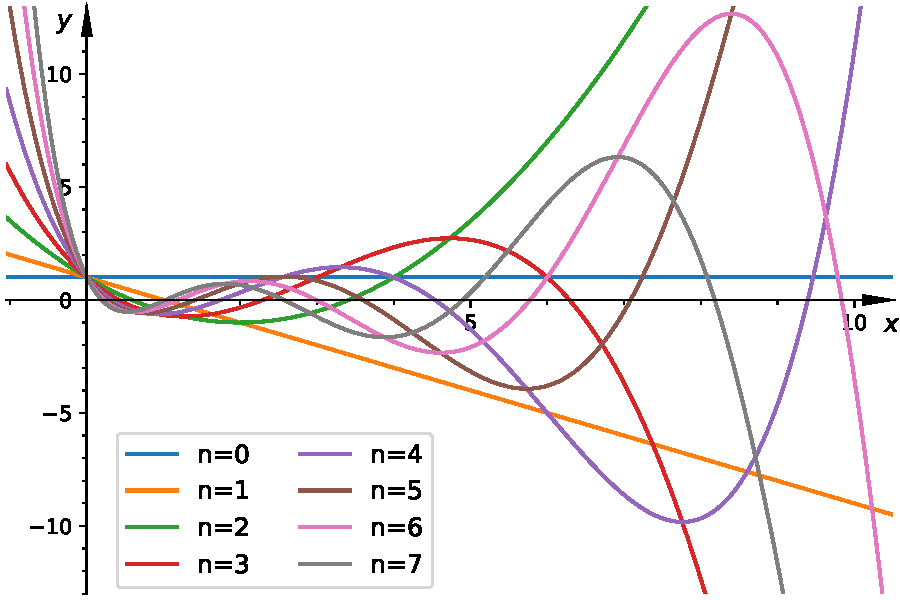
\includegraphics[width=0.7\textwidth]{%
    papers/laguerre/images/laguerre_polynomes.pdf%
}
\caption{Laguerre-Polynome vom Grad $0$ bis $7$}
\label{laguerre:fig:polyeval}
\end{figure}

% https://www.math.kit.edu/iana1/lehre/hm3phys2012w/media/laguerre.pdf
% http://www.physics.okayama-u.ac.jp/jeschke_homepage/E4/kapitel4.pdf
